\documentclass[a4paper,11pt]{article}

%\usepackage{khacommands}
\usepackage[pdftex]{graphicx}
%\usepackage{palatino}

\title{User manual for the HeadMotion progam. Version 2.0}
\author{Kjartan Halvorsen}

\begin{document}

\maketitle

\section{Introduction}
The HeadMotion program is used for computing the movement of the head of the
test subjects involved in the torticollis project. 
The program
computes the position and orientation (called \emph{pose}) of the head
as well as the velocity and acceleration. The program stores the
results in a database, together with information specific for the test
subject and the trial.

It is not possible to store the same trial twice in the database. This
is enforced by checking the timestamp of each trial. This string,
which is present in the tsv data file, gives the date and the time
(down to seconds) of when the data was collected. This timestamp must
be unique for every trial in the database. 

The data in the database can be analyzed by creating groups of trials,
and then run analyses, often comparisons, between the groups.

You start the program by double-clicking on the ``HeadMotion.bat''
icon on the desktop.

\section{User interface}
The graphical user interface contains three tabs: The Process tab, the
Search tab and the Analyze tab. The Process tab is used when adding
new trials to the database. The Search tab is used to search among the
trials in the database. The Analyze tab is used to create groups of
the trials in the database, and then run an analysis on the groups.

\subsection{The Process tab}
The tab contains a number of text fields and
socalled ``combo-boxes''. The combo-boxes store alternatives that can
be chosen for each field. See figure \ref{fig:processgui}
\begin{figure}[htbp]
  \centering
  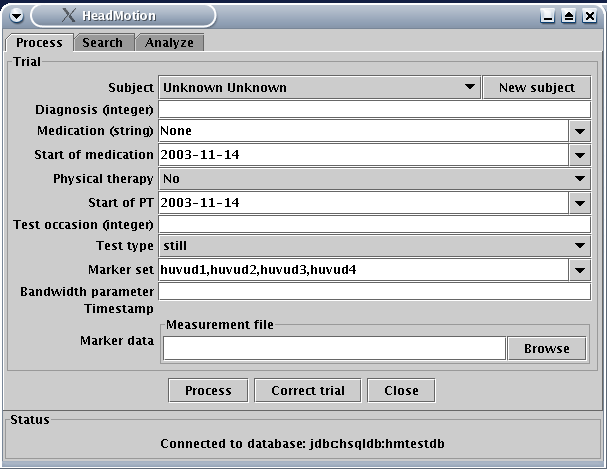
\includegraphics[width=120mm]{figures/gui_overview.png}
  \caption{Graphical user interface}
  \label{fig:processgui}
\end{figure}

Of the three buttons at the bottom, the left (``Process'') is used to
add a new trial to the database, the middle (``Correct trial'') is
used to edit the information about an existing trial, and the right
(``Close'') will close the program. 

\subsubsection{Adding a new trial to the database}
To process trials and add them to the database, follow the given
steps:
\begin{enumerate}
\item Choose the subject. To add a new subject, edit an existing or searching for a subject, press the ``Add/Edit
  subject'' button. This launches a dialog. See explenation in the next section.
\item Choose the measurement file (a .tsv file) by clicking the
  ``Browse'' button. This will launch a standard file chooser dialog.
\item Set the information about the subject and the trial:
  \begin{description}
  \item[Diagnosis] This integer represents the diagnosis. 0 would
    typically indicate a healthy person, and any other number some
    code that has to be defined.
  \item[Medication] Some standard botolinum toxins are listed.
  \item[Start of medication] Set to empty if no medication is given.
  \item[Physical therapy] Yes or no.
  \item[Start of PT]  Set to empty if no PT is prescribed.
  \item[Test occasion] 1 for the first time, 2 for the second, etc. 
  \item[Test date] Self-explanatory
  \item[Test type] This list could be expanded as new tests are
    defined.
  \item[Marker set] The names of the markers on the head. If other
    names than those suggested are used, then write the names
    separated by commas.
  \item[Bandwidth parameter] This parameter controls the
    computations. A number greater than 1 will give less smoothing of
    the results. However, the high frequency noise in the data will
    start to dominate the calculated velocity and acceleration.
  \end{description}
\item Click ``Process'' to compute the movement and add the results to
  the database.
\item The results will be presented in a separate plot window. A dialog
  will also pop-up, and ask you to save to a text file. If you want
  the results in a text file for importing to excel, then enter a
  suitable name and click ``Save''. Otherwise, just cancel: the data
  is saved in the database in any case.
\item If you want to print the results directly, there is a print
  button on the plot window. The quality is not perfect. I will try to
  improve it later.
\end{enumerate}

\subsubsection{Adding, searching and editing subject information}
Figure \ref{fig:subjectgui} shows the dialog for handling information on the test subjects.
  \begin{figure}[htbp]	
    \centering	
    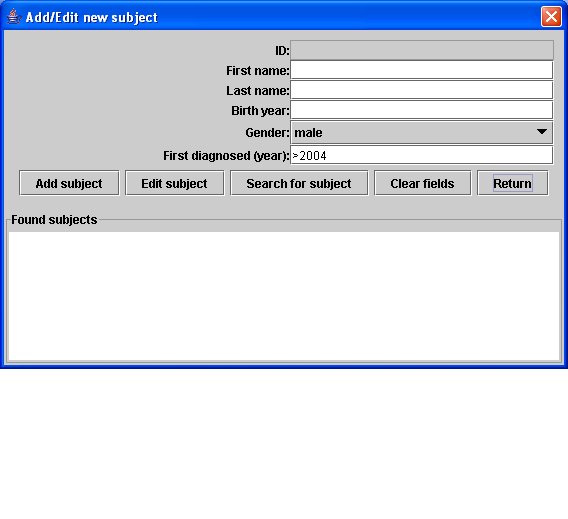
\includegraphics[width=140mm]{figures/subjectgui.png}
    \caption{Dialog for handling the subject information}
    \label{fig:subjectgui}
  \end{figure}
To add a new subject to the database, simply fill out the form and
press ``Add''. To search for a subject, type in search criteria in the
fields and press ``Search for subject''. Here are some examples of how
to set search criteria:
\begin{itemize}
\item First or last name: The character ``\%'' can be used as a wild
card, so if you write ``A\%'' for first name, you search for all
subjects with first name starting with A.
\item Birth year: Use $>1950$ to search for subjects born after 1950.
\item First diagnosed: Use $<2004$ to search for subjects diagnosed
before 2004.
\end{itemize}

\subsubsection{Editing the information for an existing trial}
Sometimes the information for a specific trial needs to be
changed. An example of this is when artefacts in the data make the
trial unfit for further analysis. A trial cannot be deleted from the
database, but we can make sure that it will not show up when we define
groups from the trials (see the section on the Analyze tab). 

To open a specific trial to edit, you first need to find it by using
the Search tab (see sectione below). You can see that a trial is ready
to be edited by checking that the Timestamp field has a value. Change
the information for the trial, and then click on ``Correct trial'' to
save the changes to the database. To continue with the example above,
change Test occasion to a negative number. It will then be easy to
avoid the trial when defining groups. It is a good idea in this case
to set the Test occasion to $-2$ if the number was 2, and so on, in
order to remember what it originally was.

\subsection{The Search tab}
The Search tab is used for searching among the trials in the
database. Figure \ref{fig:searchgui} shows the interface. In the
displayed example, the database has been searched for healthy subjects
(Diagnosis set to ``=0''), trials from the first test day (Test
occasion set to ``=1'') and trials with the head kept still (Test type
set to ``still''). 
  \begin{figure}[htbp]
    \centering
    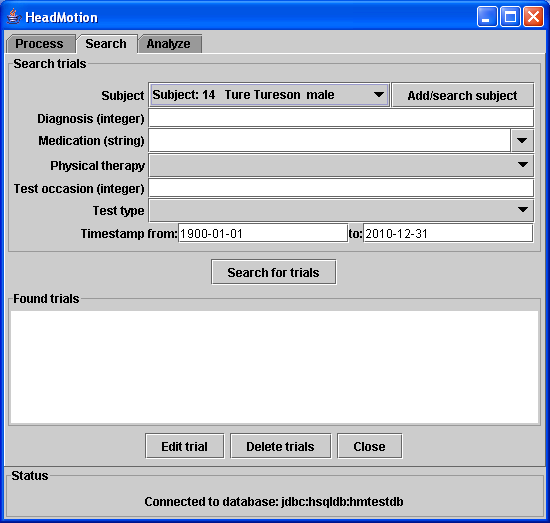
\includegraphics[width=120mm]{figures/searchgui.png}
    \caption{The Search tab}
    \label{fig:searchgui}
  \end{figure}

A trial may be edited by selecting it in the list, and then click the
``Edit trial'' button. The information about the trial will then be
presented in the Process tab.

\subsection{The Analyze tab}
The tab conists of a list of groups, with buttons that will add a new
group, edit an existing one, or delete selected groups. See Figure
\ref{fig:analyzegui}. The tab also contains a drop down list with
different types of analyses that can be run on the groups. The left of
the two buttons on the bottom will start the analysis. The right
button will close the program.
  \begin{figure}[htbp]
    \centering
    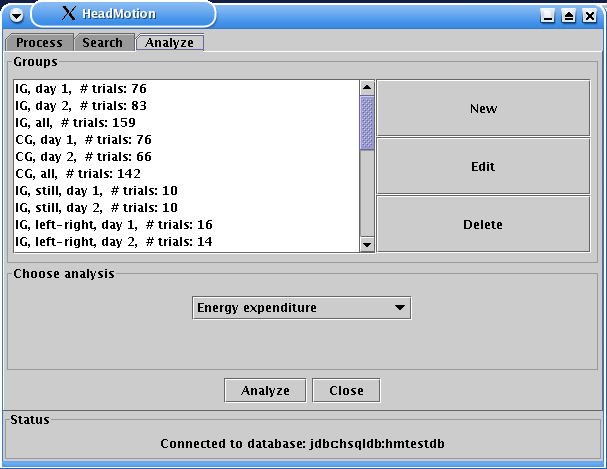
\includegraphics[width=120mm]{figures/analyzegui.png}
    \caption{The Analyze tab}
    \label{fig:analyzegui}
  \end{figure}

\subsubsection{Adding or editing a group}
Upon clicking the New button, a dialog pops up (Figure
\ref{fig:groupdescription}). Enter a descriptive name for the group
and click OK. 
  \begin{figure}[htbp]
    \centering
    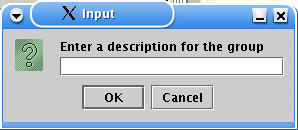
\includegraphics[width=60mm]{figures/groupdescription.png}
    \caption{The new goup dialog}
    \label{fig:groupdescription}
  \end{figure}

A new window pops up, in which you define the trials that
should go in the group. Clicking Edit in the Analyze tab will bring
you directly to this window. Figure \ref{fig:searchgroupgui} shows the
interface for a case when the group already contains a set of
trials. Note that the name of the group appears on the window's title bar.
  \begin{figure}[htbp]
    \centering
    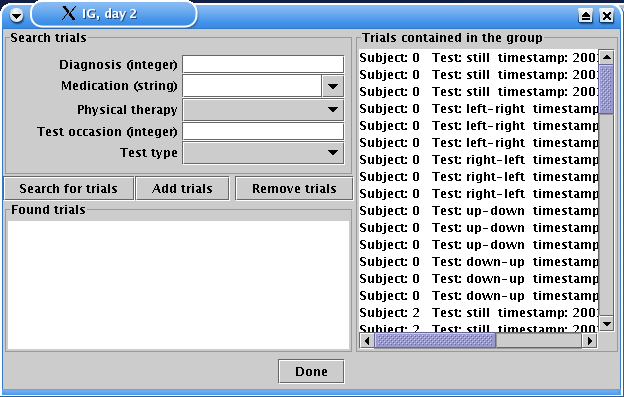
\includegraphics[width=120mm]{figures/searchgroupgui.png}
    \caption{The interface for defining the trials that go into a group}
    \label{fig:groupdescription}
  \end{figure}
The interface works very much like the Search tab. The upper left
frame, titled ``Search trial'' is used to define search criteria. If
all fields (Diagnosis, Medication, Physical therapy, Test occasion and
Test type) are left with no values set or chosen, then a search will
return all the trials in the database. If, for instance, Test type is
set to ``still'', then a search will return all trials with the test
subject keeping the head still. If, furtheron, Diagnosis is set to
``>0'', then a search will return all patient trials with the head
still. 

The Diagnosis and Test occasion fields work in the same way. Define a
criterion by writing either of ``='', ``<'' or ``>'', followed by an
integer. Remember that healthy control subjects have diagnosis
0. Writing ``=0'' in the Diagnosis field will give trials for control
subjects only. 

The trials that are found in a search will appear in the list on the
lower left of the interface, titled ``Found trials''. To add trials
from this group to the group you have to first select them, and then
click the ``Add trials'' button. The selected trials will appear on
the list to the right. Trials that are already there will not be
added, so there are no risk of duplicating trials in the group. 

To remove trials from the group, select the trials in the right side
list, and then click the Remove trials button.

Click Done when you are satisfied with the contents of your group. If
the group is empty (no trials on the right side list), then it is
discarded.  

\subsubsection{Running an analysis}
The two most important analyses in the current version (1.0), are
``Energy expenditure'' and ``Energy expenditure test-retest''. To run
either of the analyses, choose two groups from the list, pick the
analysis and click ``Analyze''. Depending on the size of the groups,
the analysis may take quite some time (several minutes). 

The analyses:
\begin{description}
\item[Energy expenditure] Comparison of the Energy Expenditure Index
  between two independent groups 
  using the Wilcoxon two sample test. The EEI is computed for each
  trial in the groups. Before running the Wilcoxon test, each 
  group is \emph{consilidated}. By this is meant that all the trials in
  the group that is from the same test subject and the same test type
  are averaged. The hypothesis test is performed on the averages. 
  The result from the test is presented in a
  dialog (Figure \ref{fig:eeresult}) and the EEI valuse are plotted
  on a logarithmic scale (Figure \ref{fig:eeplot}).
  \begin{figure}[htbp]
    \centering
    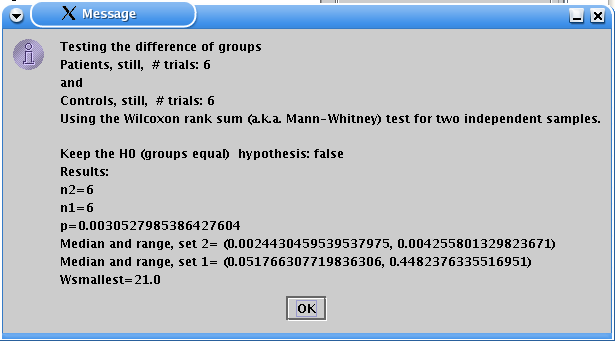
\includegraphics[width=60mm]{figures/eeresults.png}
    \caption{The results from an Energy expenditure analysis.}
    \label{fig:eeresult}
  \end{figure}
  \begin{figure}[htbp]
    \centering
    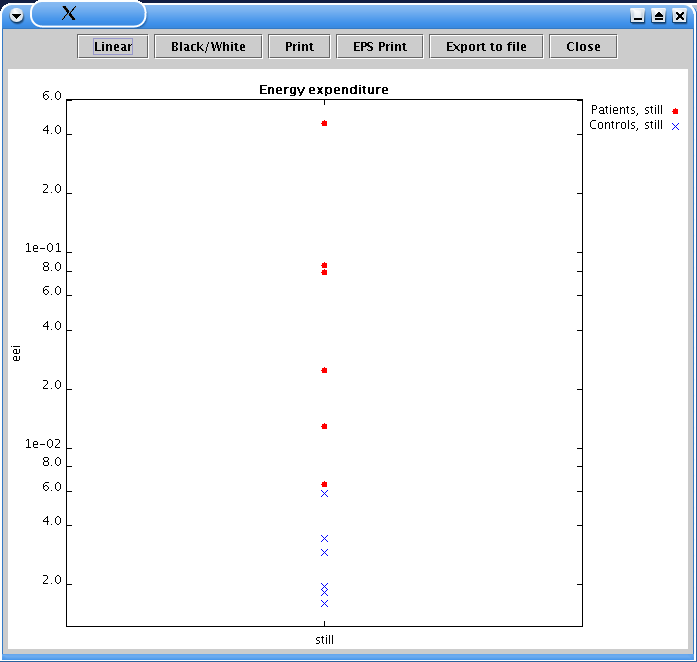
\includegraphics[width=120mm]{figures/eeplot.png}
    \caption{Resulting Energy Expenditure Index plotted.}
    \label{fig:eeplot}
  \end{figure}
\item[Energy expenditure test-retest] Comparison of EEI between two
  groups with matching trials. Uses the Wilcoxon matched-pairs signed
  rank test. The trials are matched up if they are from the same test
  subject and the same test type. The results are presented as in
  Figures \ref{fig:eetestretest} and \ref{fig:eetestretestplot}.
  \begin{figure}[htbp]
    \centering
    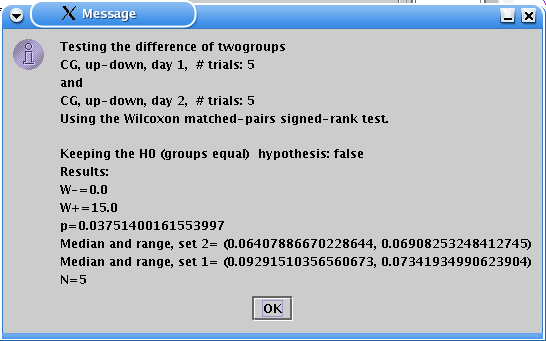
\includegraphics[width=60mm]{figures/eetestretestresult.png}
    \caption{The results from an Energy expenditure test-retest analysis.}
    \label{fig:eetestretest}
  \end{figure}
  \begin{figure}[htbp]
    \centering
    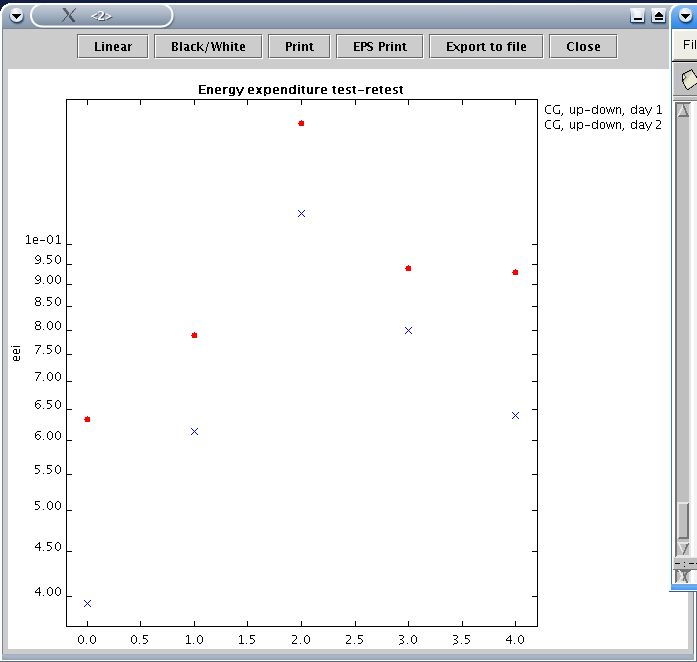
\includegraphics[width=120mm]{figures/eetestretestplot.png}
    \caption{Pairs of matched Energy Expenditure Index values are plotted.}
    \label{fig:eetestretestplot}
  \end{figure}

\item[Diagnose] Goes through the trials in a group and checks for
  unexpected large values of EEI. If found, the data for the trials
  are plotted. 

\item[Edit the database entries] Will display all the trials in the
  selected group in the list in the Search tab (Figure
  \ref{fig:searchgui}). 

\item[Print info] Prints out on the comman prompt the subject ID
  number, the Test type, and the   timestamp for each trial in the group. 
\end{description}
\end{document}
